\documentclass{beamer}
\usepackage{ragged2e}
\usepackage{amsmath,amssymb}

\title{Modelos Generativos Profundos}
\subtitle{Clase 23: Modelos de difusión (parte III)}
\author{Fernando Fêtis Riquelme}
\institute{
    Facultad de Ciencias Físicas y Matemáticas\\
    Universidad de Chile
}
\date{Primavera, 2025}
\titlegraphic{\hfill
\includegraphics[height=1.2cm]{images/fcfm}}

\usetheme{metropolis}
\setbeamercovered{transparent}

\newcommand{\R}{\mathbb{R}}
\newcommand{\N}{\mathbb{N}}
\newcommand{\Z}{\mathbb{Z}}
\newcommand{\pr}{\mathbb{P}}
\newcommand{\argmax}{\operatorname{argmax}}
\newcommand{\argmin}{\operatorname{argmin}}
\newcommand{\insertimage}[2]{
    \begin{center}
        \includegraphics[width=#2\textwidth]{images/#1}
    \end{center}
}
\setlength{\leftmargini}{0em}
\renewcommand{\raggedright}{\leftskip=0pt \rightskip=0pt plus 0cm}

\justifying

\begin{document}

\begin{frame}
    \titlepage
\end{frame}

\begin{frame}{Clase de hoy}
    \tableofcontents
\end{frame}

\section{Generación condicional y guidance}

\begin{frame}{Idea general}
    Al igual que toda red bayesiana, un modelo de difusión puede ser extendido para aprender \textbf{distribuciones condicionales} $p_\text{data}(x|y)$, donde $y\sim p(y)$ es alguna variable condicionante. Para esto, es suficiente considerar un proceso backward condicional,
    \begin{equation*}
        p_\theta(x_{0:T}|y)=p(x_T)\prod_{t=1}^T p_\theta(x_{t-1}|x_t,y),
    \end{equation*}
    donde ahora las transiciones $p_\theta(x_{t-1}|x_t, y)\sim\mathcal{N}\left(\mu_\theta(x_t,t, y),\sigma_q^2(t)\operatorname{I}_D\right)$ dependen del factor condicionante $y$.

    En la práctica, esto se logra considerando a $y$ como una entrada adicional a la red neuronal $\mu_\theta$, la cual puede ser inyectada de diversas formas, dependiendo de la naturaleza de $y$.
\end{frame}

\begin{frame}{Idea general}
    En su forma más simple, $y\in\R^C$ es un vector, por ejemplo:
    \begin{itemize}
        \item Un vector one-hot que indica una clase.
        \item Un embedding de texto obtenido a partir de un modelo preentrenado (p.g. CLIP o BERT).
    \end{itemize}
    Si bien una estrategia simple es concatenar $y$ a la entrada de la red neuronal, en la práctica se utilizan técnicas más sofisticadas.

    Un método usual consiste en sumar el embedding temporal (asociado al tiempo de denoising $t\in\{1,\ldots,T\}$) y el embedding de la condición $y\in\R^D$, para luego inyectar esta suma en la red neuronal mediante \textbf{modulaciones tipo FiLM}.
\end{frame}

\begin{frame}{Modelos de embedding para texto}
    Para obtener una representación vectorial de un prompt, se pueden utilizar modelos preentrenados como \textbf{BERT} o \textbf{CLIP}.
    \begin{center}
        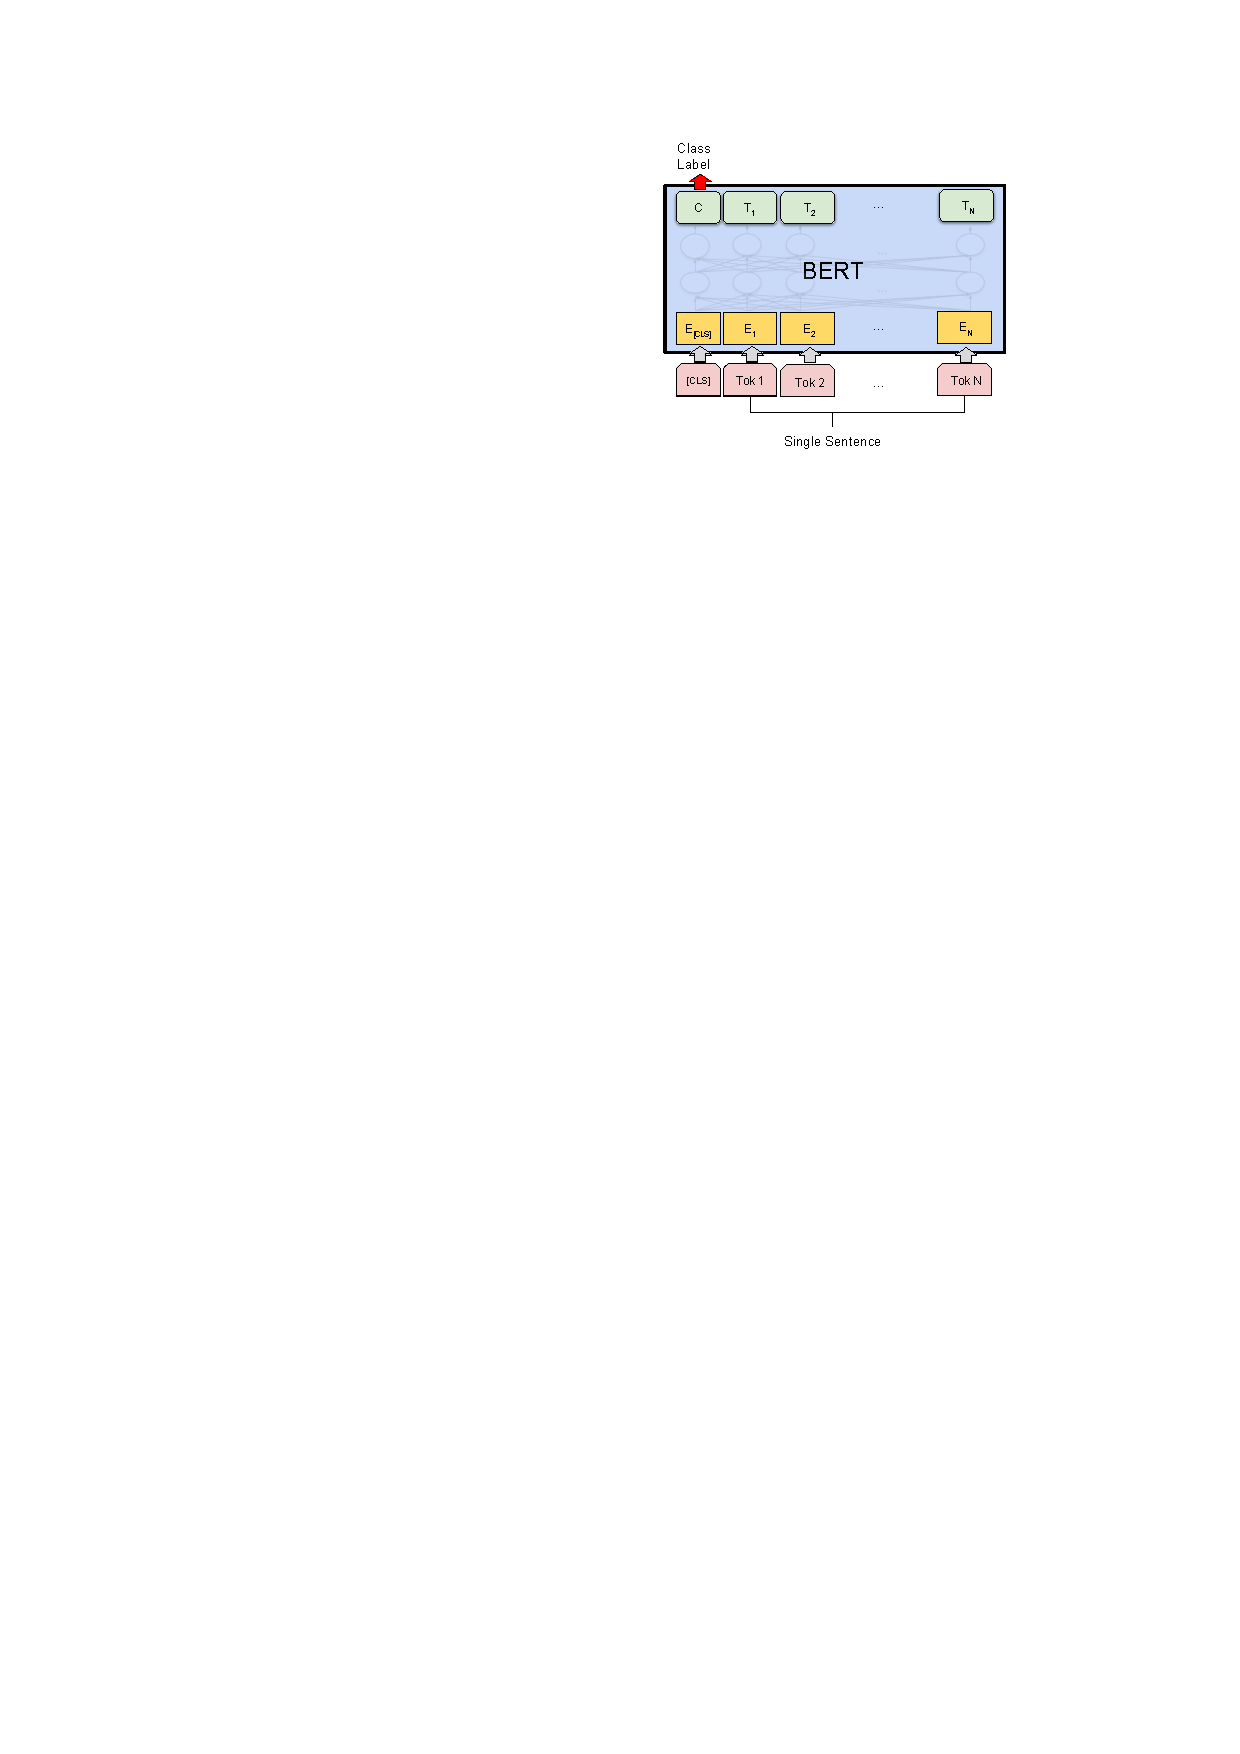
\includegraphics[width=0.4\textwidth]{images/bert}
        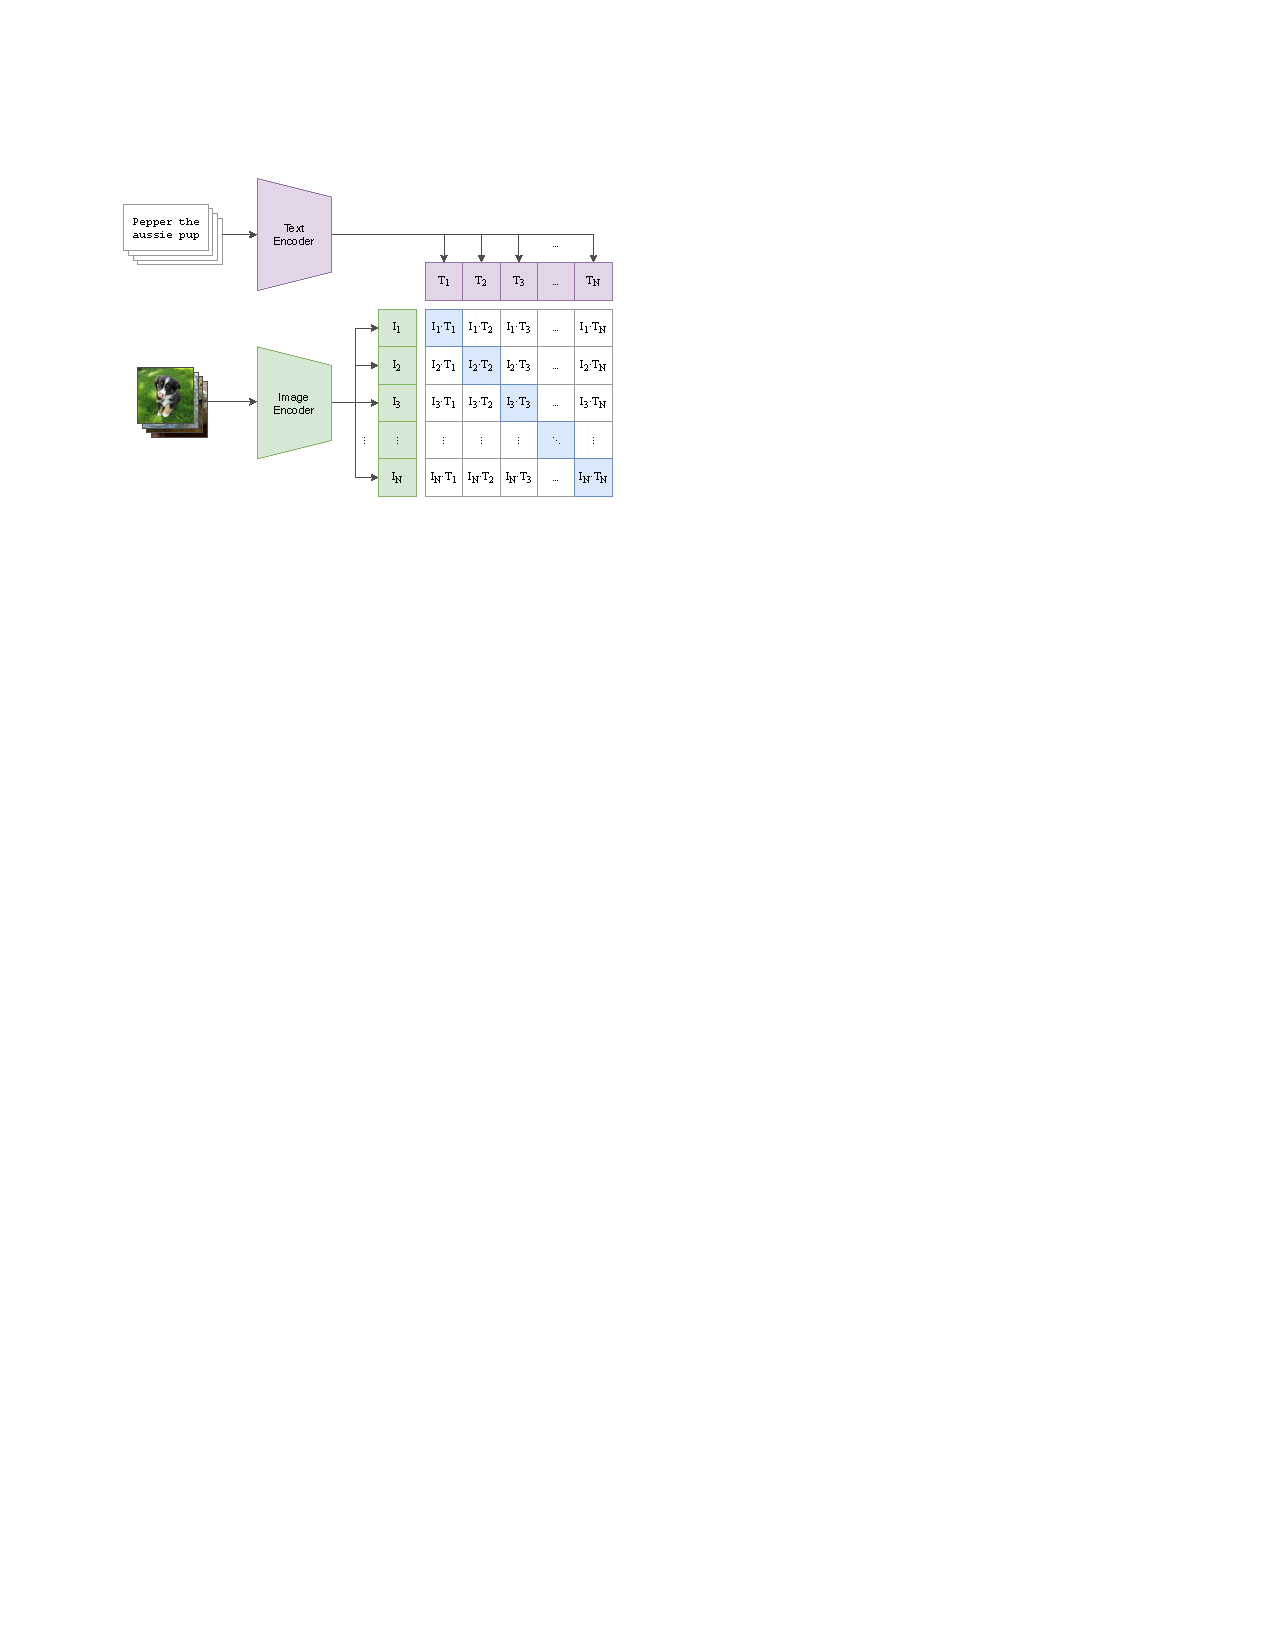
\includegraphics[width=0.5\textwidth]{images/clip}
    \end{center}
    Sin embargo, solo inyectar un embedding del prompt suele ser insuficiente para obtener una buena generación condicional. La técnica de \textbf{guidance} permite darle mayor peso a la condición durante el proceso de generación.
\end{frame}

\begin{frame}{Reparametrización score-prediction}
    Un modelo de difusión entrena una red neuronal $\mu_\theta(x_t,t)$ para predecir la media $\mu_q(x_0,x_t,t)$ de la distribución $q(x_{t-1}|x_t,x_0)$. La clase pasada se vieron formas equivalentes para esta cantidad:
    \vspace{-0.5cm}
    \begin{itemize}
        \item $\mu_q(x_0,x_t,t)=\left(\frac{c_1(t)}{\sqrt{\bar\alpha_t}}+c_2(t)\right)x_t- \frac{c_1(t)\sqrt{1-\bar\alpha_t}}{\sqrt{\bar\alpha_t}}\epsilon(x_0,x_t,t)$
        \item $\mu_q(x_0,x_t,t) = \left(\frac{c_1(t)}{\sqrt{\bar\alpha_t}}+c_2(t)\right)x_t+ \frac{c_1(t)(1-\bar\alpha_t)}{\sqrt{\bar\alpha_t}}\nabla_{x_t}\log q(x_t)$
    \end{itemize}
    En particular, se tiene que
    \begin{equation*}
        \epsilon(x_0,x_t,t) = -\sqrt{1-\bar\alpha_t}\nabla_{x_t}\log q(x_t),
    \end{equation*}
    por lo que aprender el ruido o el score es, en esencia, el mismo problema.

    Sin embargo, la formulación de score permite descomponer la señal de la condición sobre el proceso de generación.
\end{frame}

\begin{frame}{Classifier guidance}
    Dada la equivalencia anterior, un DM condicional necesita aprender el score condicional $\nabla_{x_t}\log q(x_t|y)$. Usando la regla de Bayes:
    \begin{equation*}
        \underbrace{\nabla_{x_t}\log q(x_t|y)}_{\text{DM condicional}} = \nabla_{x_t}\log q(y|x_t) + \underbrace{\nabla_{x_t}\log q(x_t)}_{\text{DM incondicional}}
    \end{equation*}
    En consecuencia, si se conoce $\nabla_{x_t}\log q(y|x_t)$, se puede realizar generación condicional utilizando un DM incondicional.

    Esta cantidad puede ser obtenida usando diferenciación automática sobre un \textbf{clasificador} entrenado para predecir $q(y|x_t)$.
\end{frame}

\begin{frame}{Classifier guidance}
    Más aún, es posible amplificar el efecto del condicionamiento utilizando un factor de escala $s\geq1$:
    \begin{equation*}
        \nabla_{x_t}\log \tilde q(x_t|y) = s\cdot\nabla_{x_t}\log q(y|x_t) + \nabla_{x_t}\log q(x_t).
    \end{equation*}
    Esta ponderación puede interpretarse como una disminución de \textbf{temperatura}, similar a lo que se hace en un LLM:
    \begin{equation*}
        \tilde q(x_t|y) \propto q(y|x_t)^s q(x_t).
    \end{equation*}
    Esta técnica se denomina \textbf{classifier guidance}, y permite darle mayor peso a la condición $y$ (usualmente un prompt o etiqueta de clase) durante el proceso de generación.
\end{frame}

\begin{frame}{Classifier-free guidance}
    Una limitación de la técnica anterior es que requiere entrenar un clasificador adicional $q(y|x_t)$, lo cual puede ser costoso.

    Una alternativa más eficiente se obtiene al notar que
    \begin{equation*}
        \nabla_{x_t}\log q(y|x_t) = \nabla_{x_t}\log q(x_t|y) - \nabla_{x_t},\log q(x_t).
    \end{equation*}
    por lo que se puede sustituir esta cantidad en CG para obtener
    \begin{equation*}
        \nabla_{x_t}\log \tilde q(x_t|y) = s\cdot\underbrace{\nabla_{x_t}\log q(x_t|y)}_{ \text{DM condicional}} +\, (1-s)\cdot\underbrace{\nabla_{x_t}\log q(x_t)}_{\text{DM incondicional}}.
    \end{equation*}
    Notar que se puede utilizar un mismo DM condicional para ambas cantidades ($\nabla_{x_t}\log q(x_t)$ se obtiene al considerar $y=\varnothing$).
\end{frame}

\begin{frame}{Classifier-free guidance}
    La técnica anterior se denomina \textbf{classifier-free guidance} y, a diferencia de CG, necesita entrenar un DM condicional:
    \begin{equation*}
        \nabla_{x_t}\log \tilde q(x_t|y) = s\cdot\nabla_{x_t}\log q(x_t|y) + (1-s)\cdot\nabla_{x_t}\log q(x_t).
    \end{equation*}
    Sin embargo, ya no es necesario entrenar un clasificador adicional, y se sigue teniendo la posibilidad de utilizar un guidance scale, $s\geq1$, para darle más importancia a factor condicionante.

    Por otro lado, la equivalencia $\epsilon-$score permite heredar la técnica de CFG directamente a DMs basados en $\epsilon$-prediction:
    \begin{equation*}
        \tilde\epsilon(x_t,t,y) = s\cdot\epsilon(x_t,t,y) + (1-s)\cdot\epsilon(x_t,t,\varnothing).
    \end{equation*}
    Esta es la forma más común de implementar CFG en la práctica.
\end{frame}

\begin{frame}{Classifier-free guidance}
    Generación condicional simple (izquierda) y con guidance (derecha).
    \begin{center}
        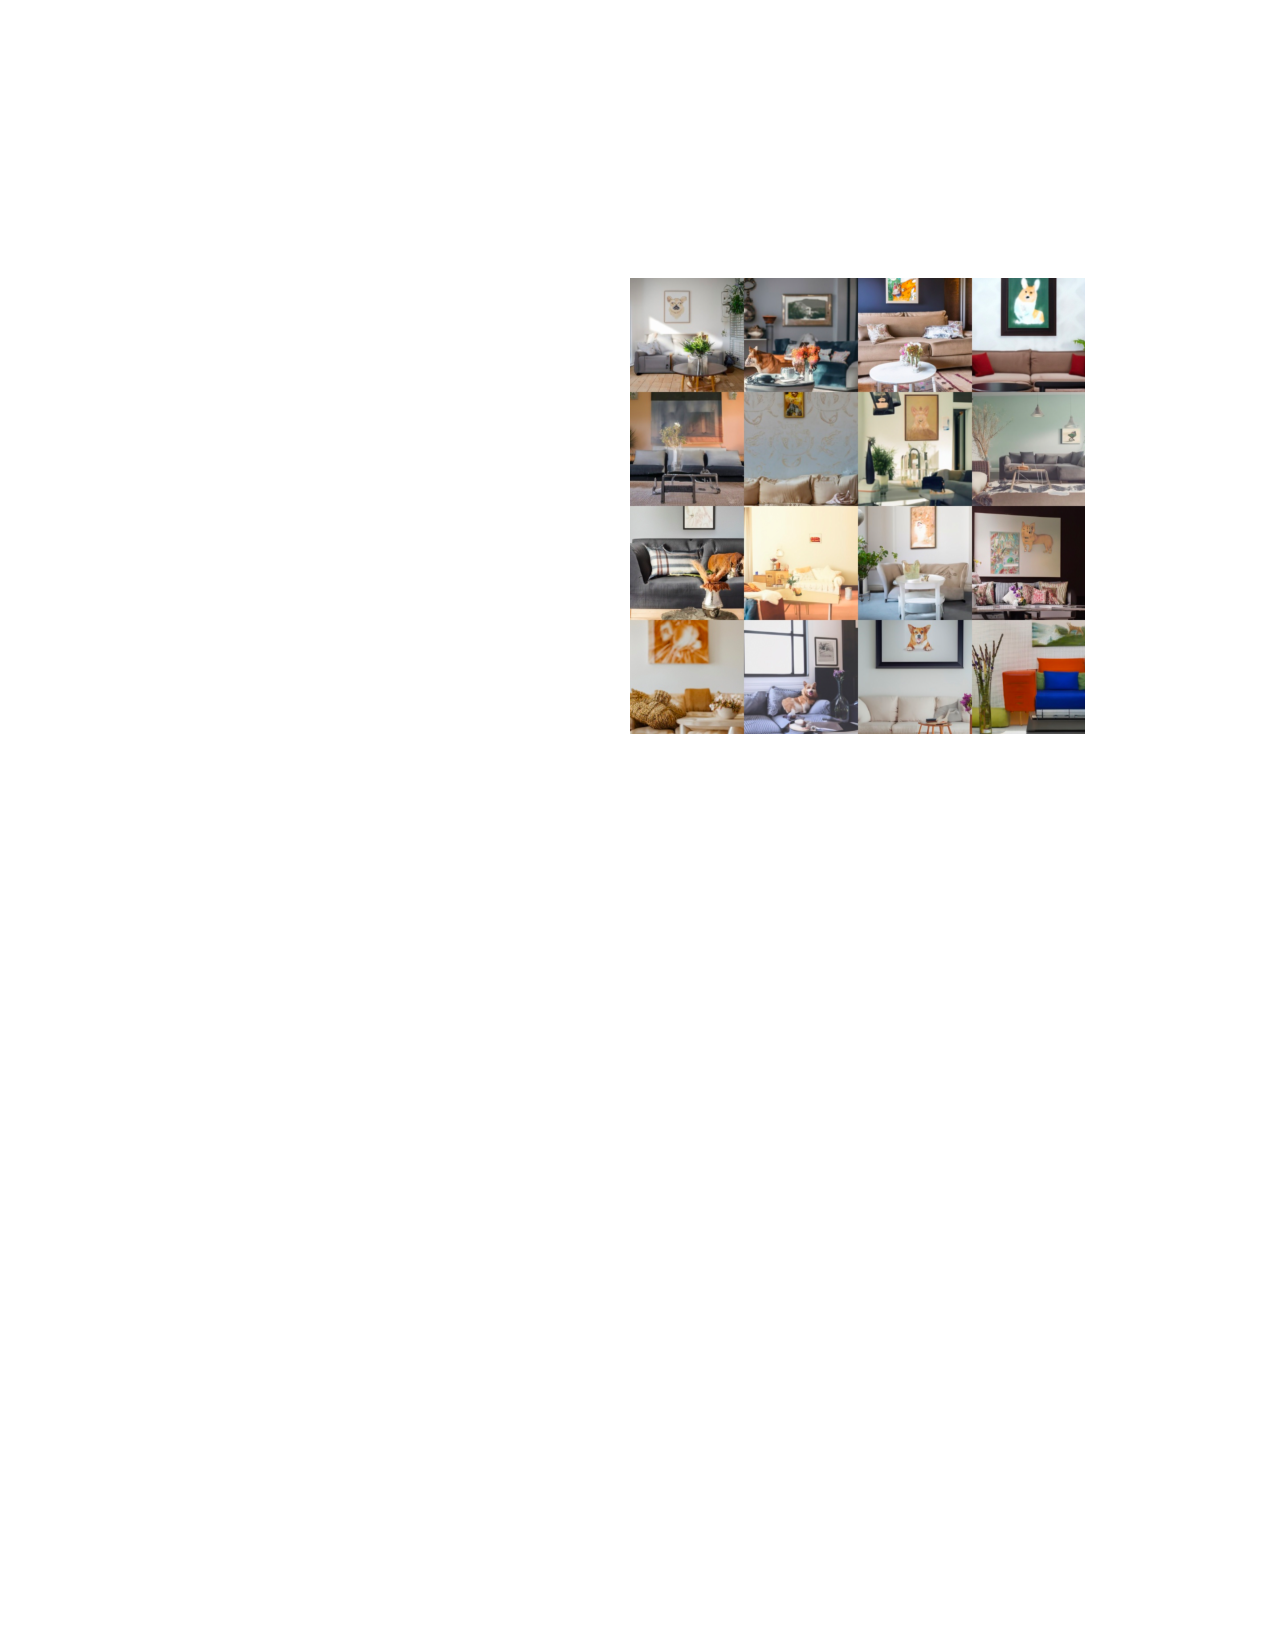
\includegraphics[width=0.45\textwidth]{images/glide_guidance}
        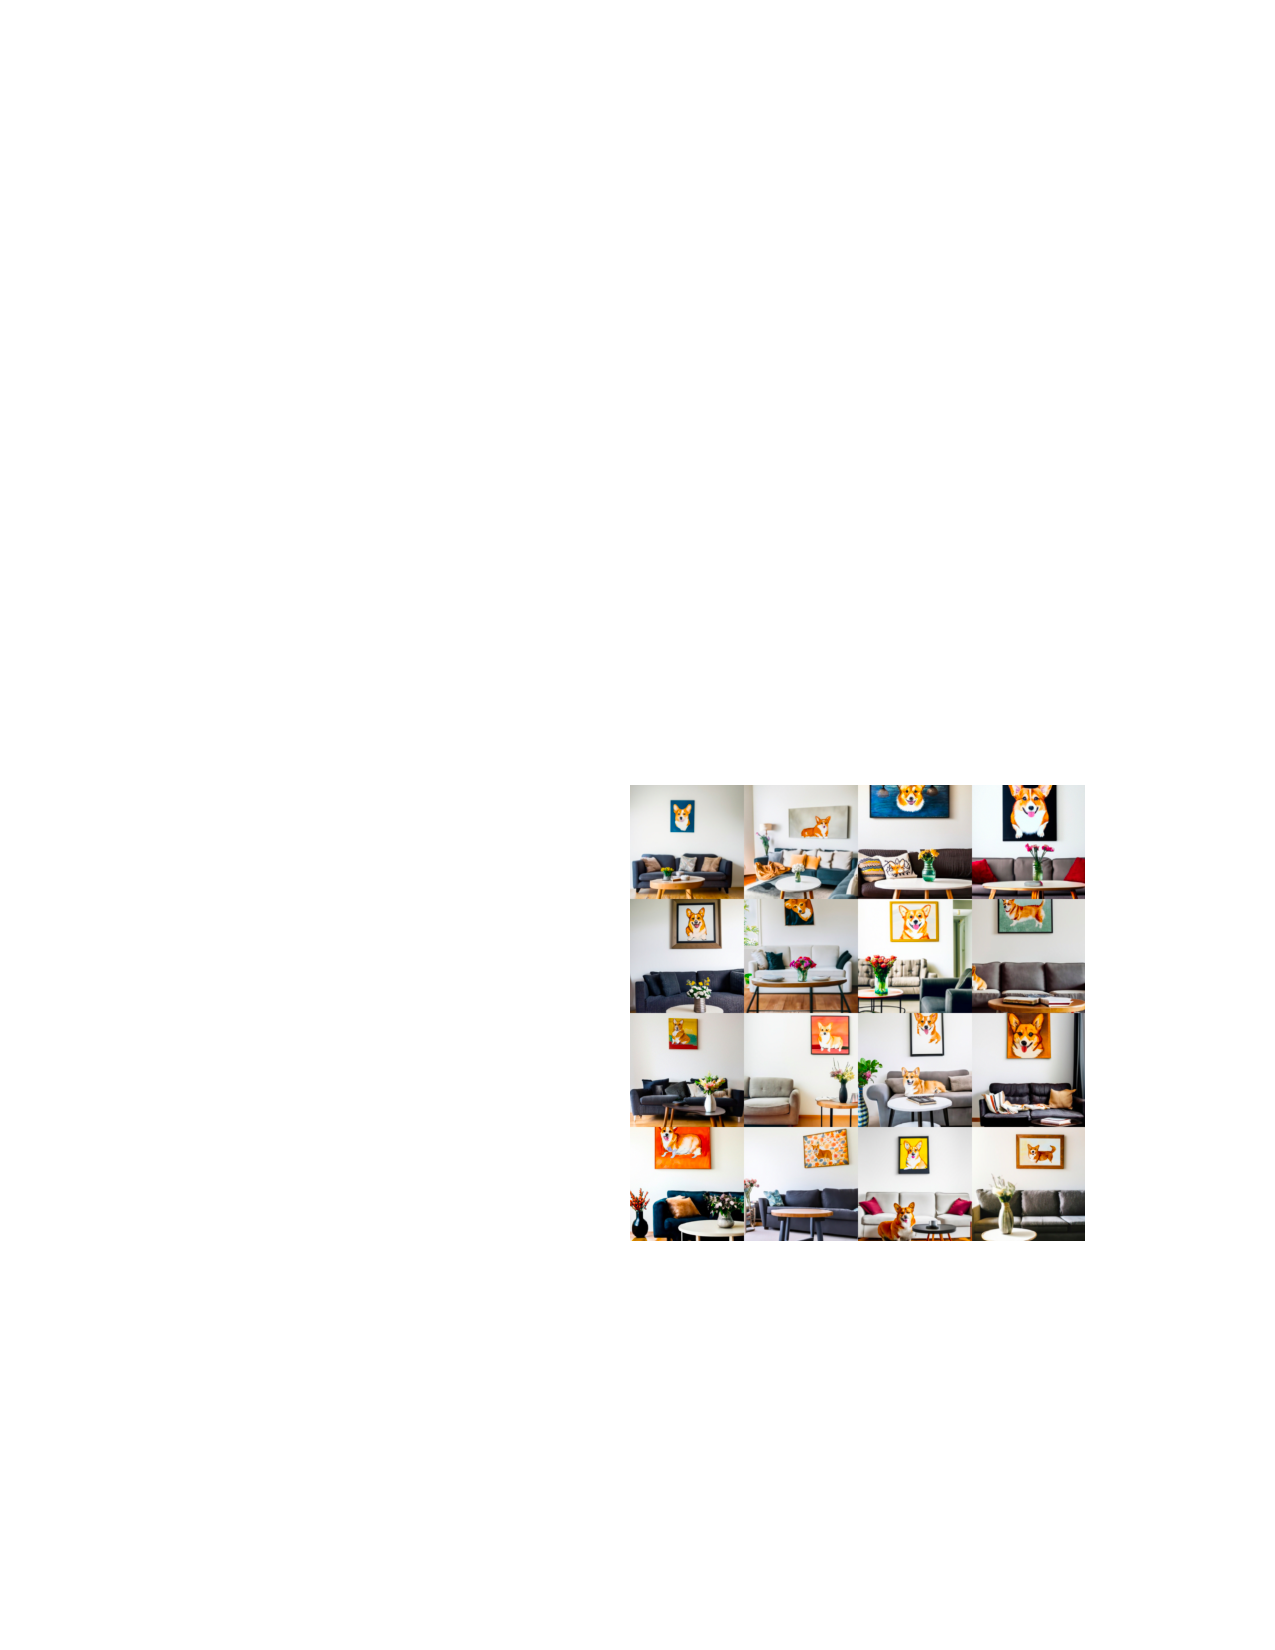
\includegraphics[width=0.45\textwidth]{images/glide_unguided}
    \end{center}
    \textbf{Prompt:} A cozy living room with a painting of a corgi on the wall above a couch and a round coffee table in front of a couch and a vase of flowers on a coffee table.
\end{frame}

\section{Arquitecturas neuronales para DMs}

\begin{frame}{U-Net}
    La arquitectura clásica en DMs es la arquitectura \textbf{U-Net con atención}. Si $\text{emb}(t)+\text{emb}(y)$ es un vector, este se inyecta en la U-Net mediante modulaciones tipo FiLM en cada bloque convolucional.
    \insertimage{attn_unet}{0.8}
\end{frame}

\begin{frame}{U-Net}
    Si $y$ es una secuencia de texto, también se puede considerar la secuencia de embeddings $\{e_1,\ldots,e_L\}$ obtenida a partir de un modelo preentrenado (p.g. T5). En este caso, se puede inyectar la información de $y$ en la U-Net mediante \textbf{atención cruzada}.
    \insertimage{cross_attn_unet}{0.7}
\end{frame}

\begin{frame}{Diffusion Transformer}
    Hoy en día, la arquitectura predominante en DMs (y flow matching) es la arquitectura \textbf{Diffusion Transformer (DiT)}, la cual puede verse como la arquitectura Vision Transformer (ViT) con capas de normalización moduladas por el tiempo y la condición.
    \insertimage{dit}{1}
\end{frame}

\section{Algunos DMs famosos}

\begin{frame}{DDPM}
    \begin{columns}
        \begin{column}{0.35\textwidth}
            \insertimage{ddpm}{1}
        \end{column}
        \begin{column}{0.65\textwidth}
            \begin{itemize}
                \item DDPM fue el primer DM moderno.
                \item Sin embargo, los DMs fueron propuestos originalmente el 2015.
                \item Es un modelo incondicional, entrenado mediante $\epsilon$-prediction.
                \item Utiliza una U-Net simple como arquitectura neuronal.
                \item Su formulación se suele considerar como la formulación (discreta) estándar.
            \end{itemize}
        \end{column}
    \end{columns}
\end{frame}

\begin{frame}{Stable Diffusion}
    \begin{itemize}
        \item Entrena un DM condicional en el espacio latente de un VAE.
        \item Utiliza una U-Net e inyecta el prompt mediante atención cruzada.
        \item Utiliza classifier-free guidance.
    \end{itemize}
    \insertimage{stable_diffusion}{0.8}
\end{frame}

\begin{frame}{Imagen}
    \begin{columns}
        \begin{column}{0.55\textwidth}
            \insertimage{imagen}{1}
        \end{column}
        \begin{column}{0.45\textwidth}
            \begin{itemize}
                \item Utiliza un esquema de cascada de DMs.
                \item Muestra que utilizar un LLM potente como text encoder es más importante que la arquitectura del DM.
                \item Se entrena con el enfoque $x_0$-prediction.
            \end{itemize}
        \end{column}
    \end{columns}
\end{frame}

\begin{frame}{DALL·E}
    \begin{itemize}
        \item Se entrena un DM (prior model) para generar un image CLIP embedding a partir del text CLIP embedding del prompt.
        \item Luego, se entrena otro DM (decoder model) para generar imágenes a partir de los image CLIP embeddings.
        \item Se puede mejorar considerablemente la calidad utilizando mejores captions durante el entrenamiento.
    \end{itemize}
    \insertimage{dalle}{0.8}
\end{frame}

\begin{frame}{Inpainting}
    La tarea de \textbf{inpainting} es un caso particular de generación condicional donde se busca completar una imagen a partir de una \textbf{máscara} que indica las regiones faltantes.
    \insertimage{inpainting}{0.8}
    Para esto, se puede realizar un sampling usual, pero manteniendo fijas las regiones no enmascaradas.
\end{frame}

\begin{frame}{Próxima clase}
    En la próxima clase.
    \begin{itemize}
        \item Uso de GPU en la nube.
        \item Adaptadores.
        \item DPO y diffusion DPO (si alcanza el tiempo).
        \item 6º control de lectura.
    \end{itemize}
\end{frame}

\begin{frame}
    \centering
    \Large{Modelos Generativos Profundos}\\
    \large{Clase 23: Modelos de difusión (parte III)}
\end{frame}

\end{document}